
\section{N-Steckverbinder}
\label{section:steckverbinder_n}
\begin{frame}%STARTCONTENT
Einsatz: \qty{2}{\metre}-Band bis in den GHz-Bereich
\begin{columns}
    \begin{column}{0.48\textwidth}
    
\begin{figure}
    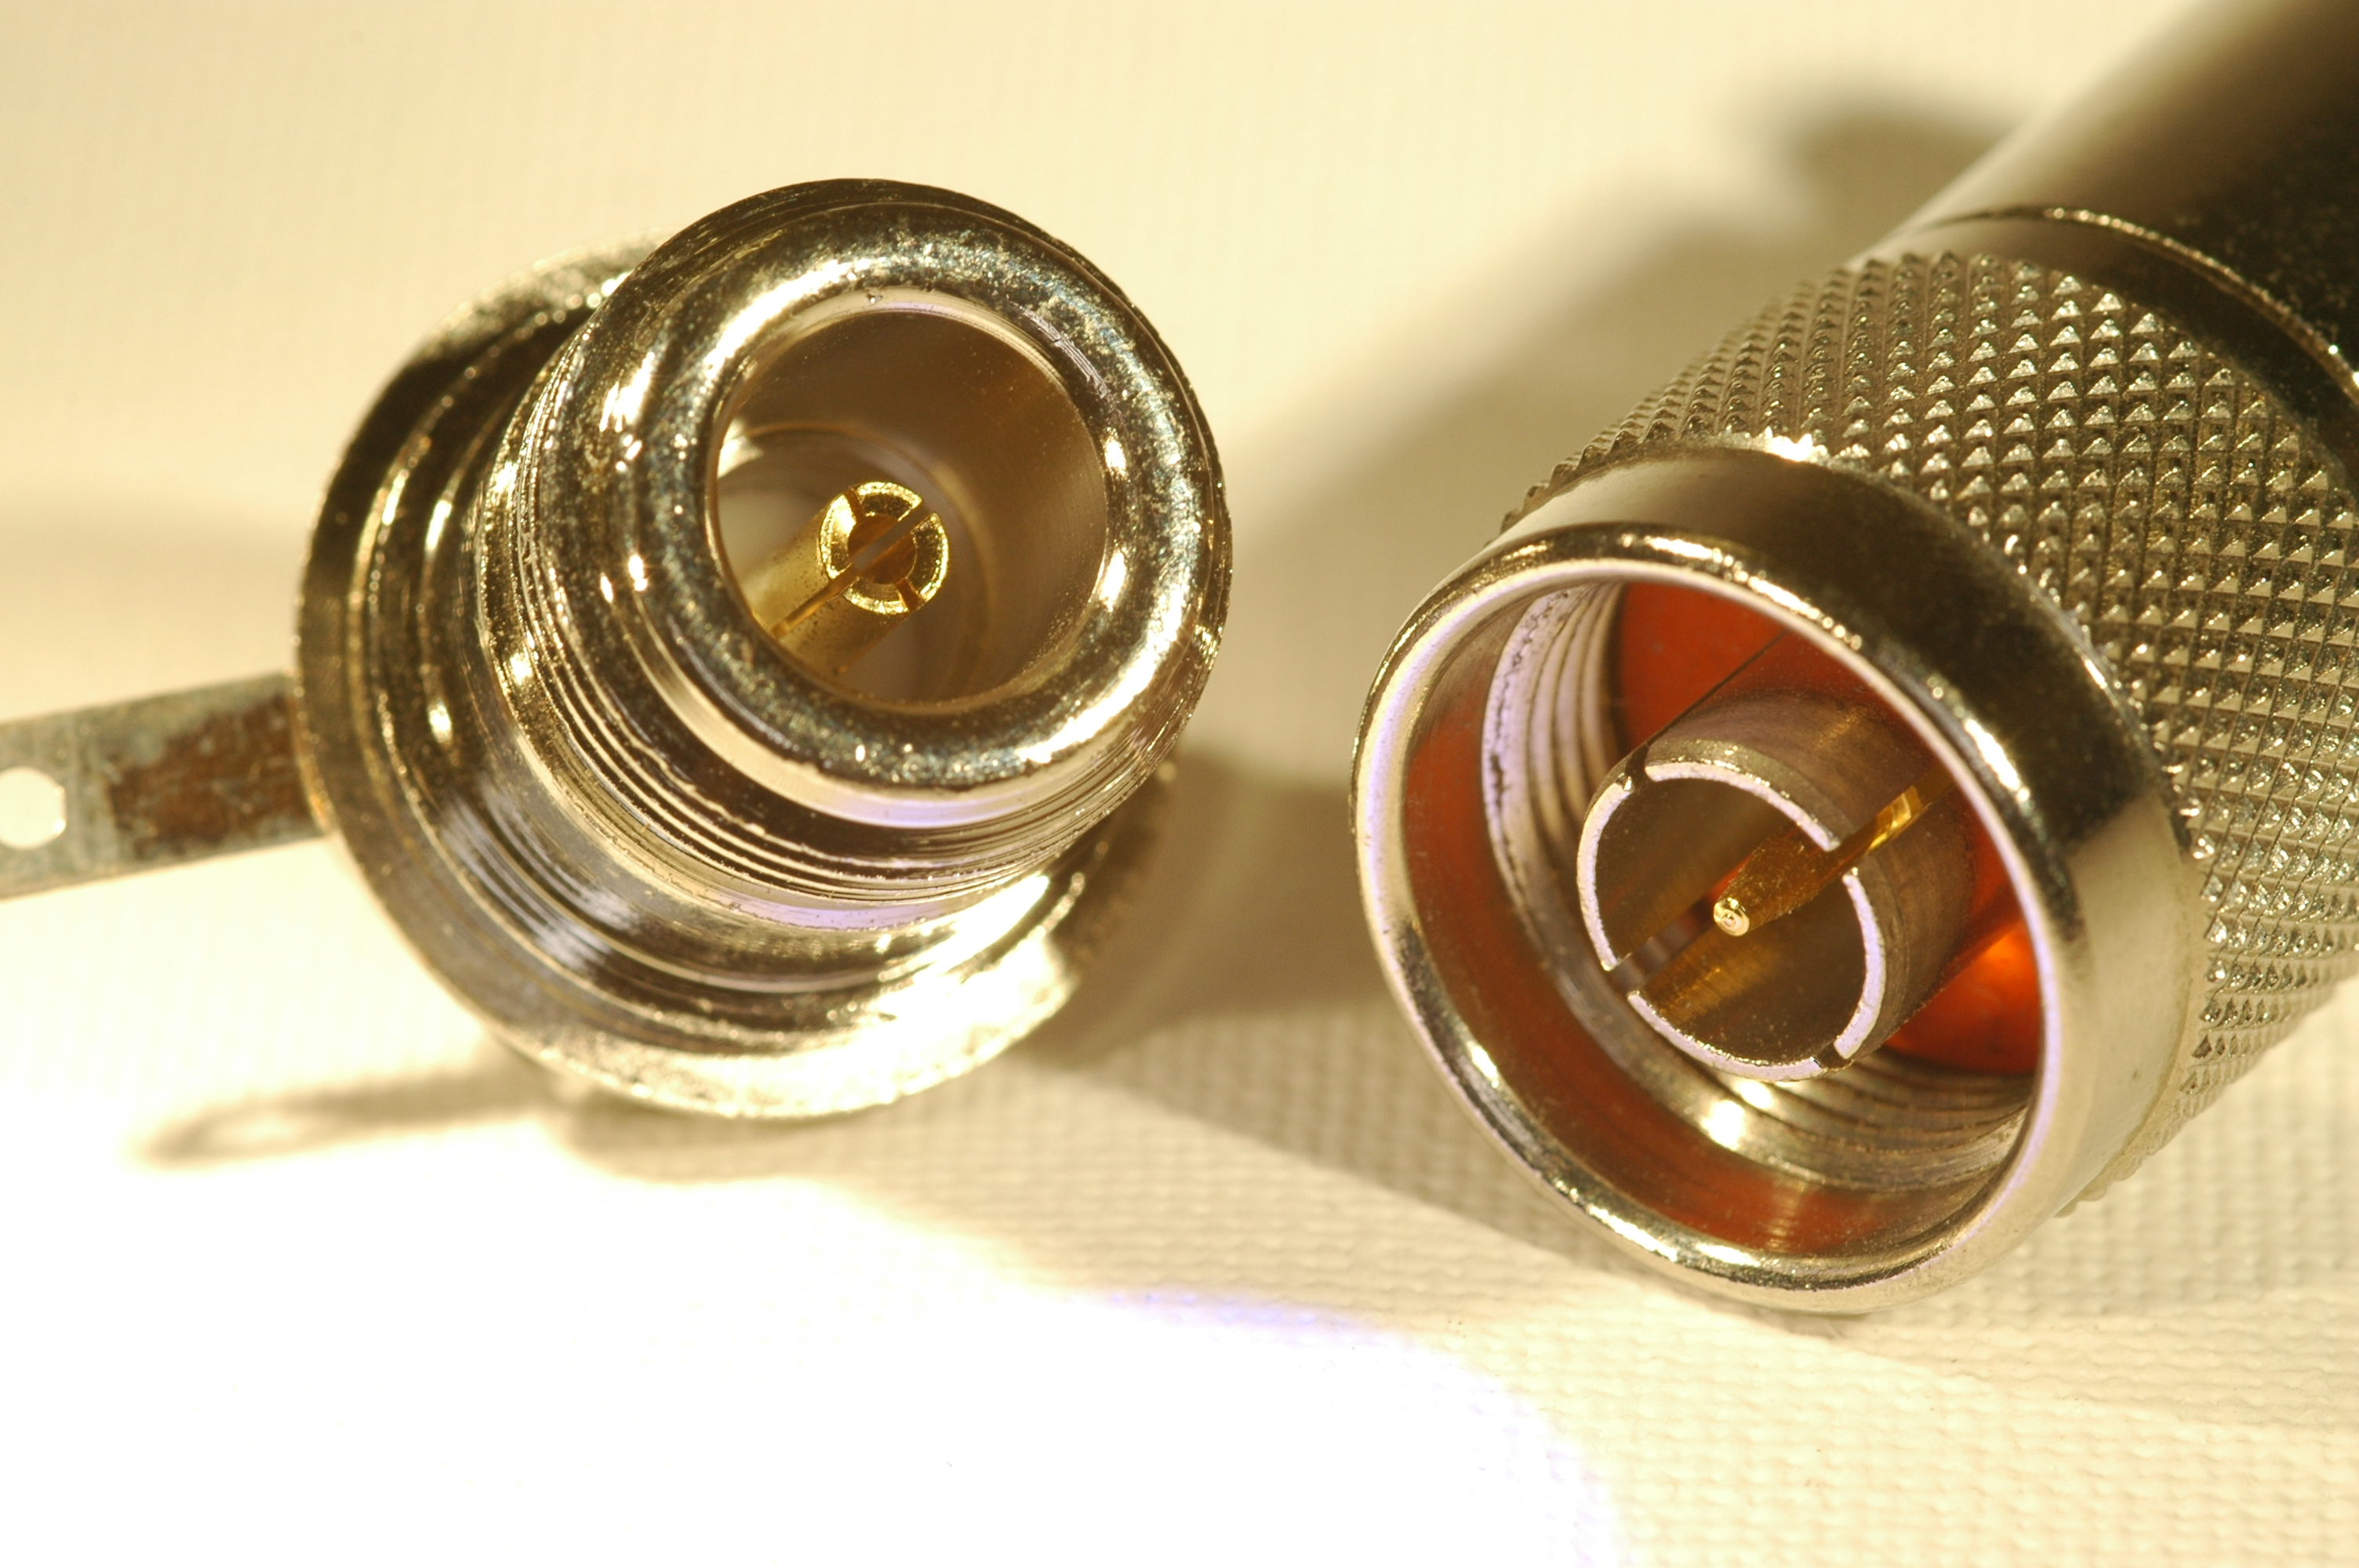
\includegraphics[width=0.85\textwidth]{foto/73}
    \caption{\scriptsize N-Einbaubuchse und N-Stecker}
    \label{n_koaxsteckverbinder_n_buchse_und_stecker}
\end{figure}

    \end{column}
   \begin{column}{0.48\textwidth}
       
\begin{figure}
    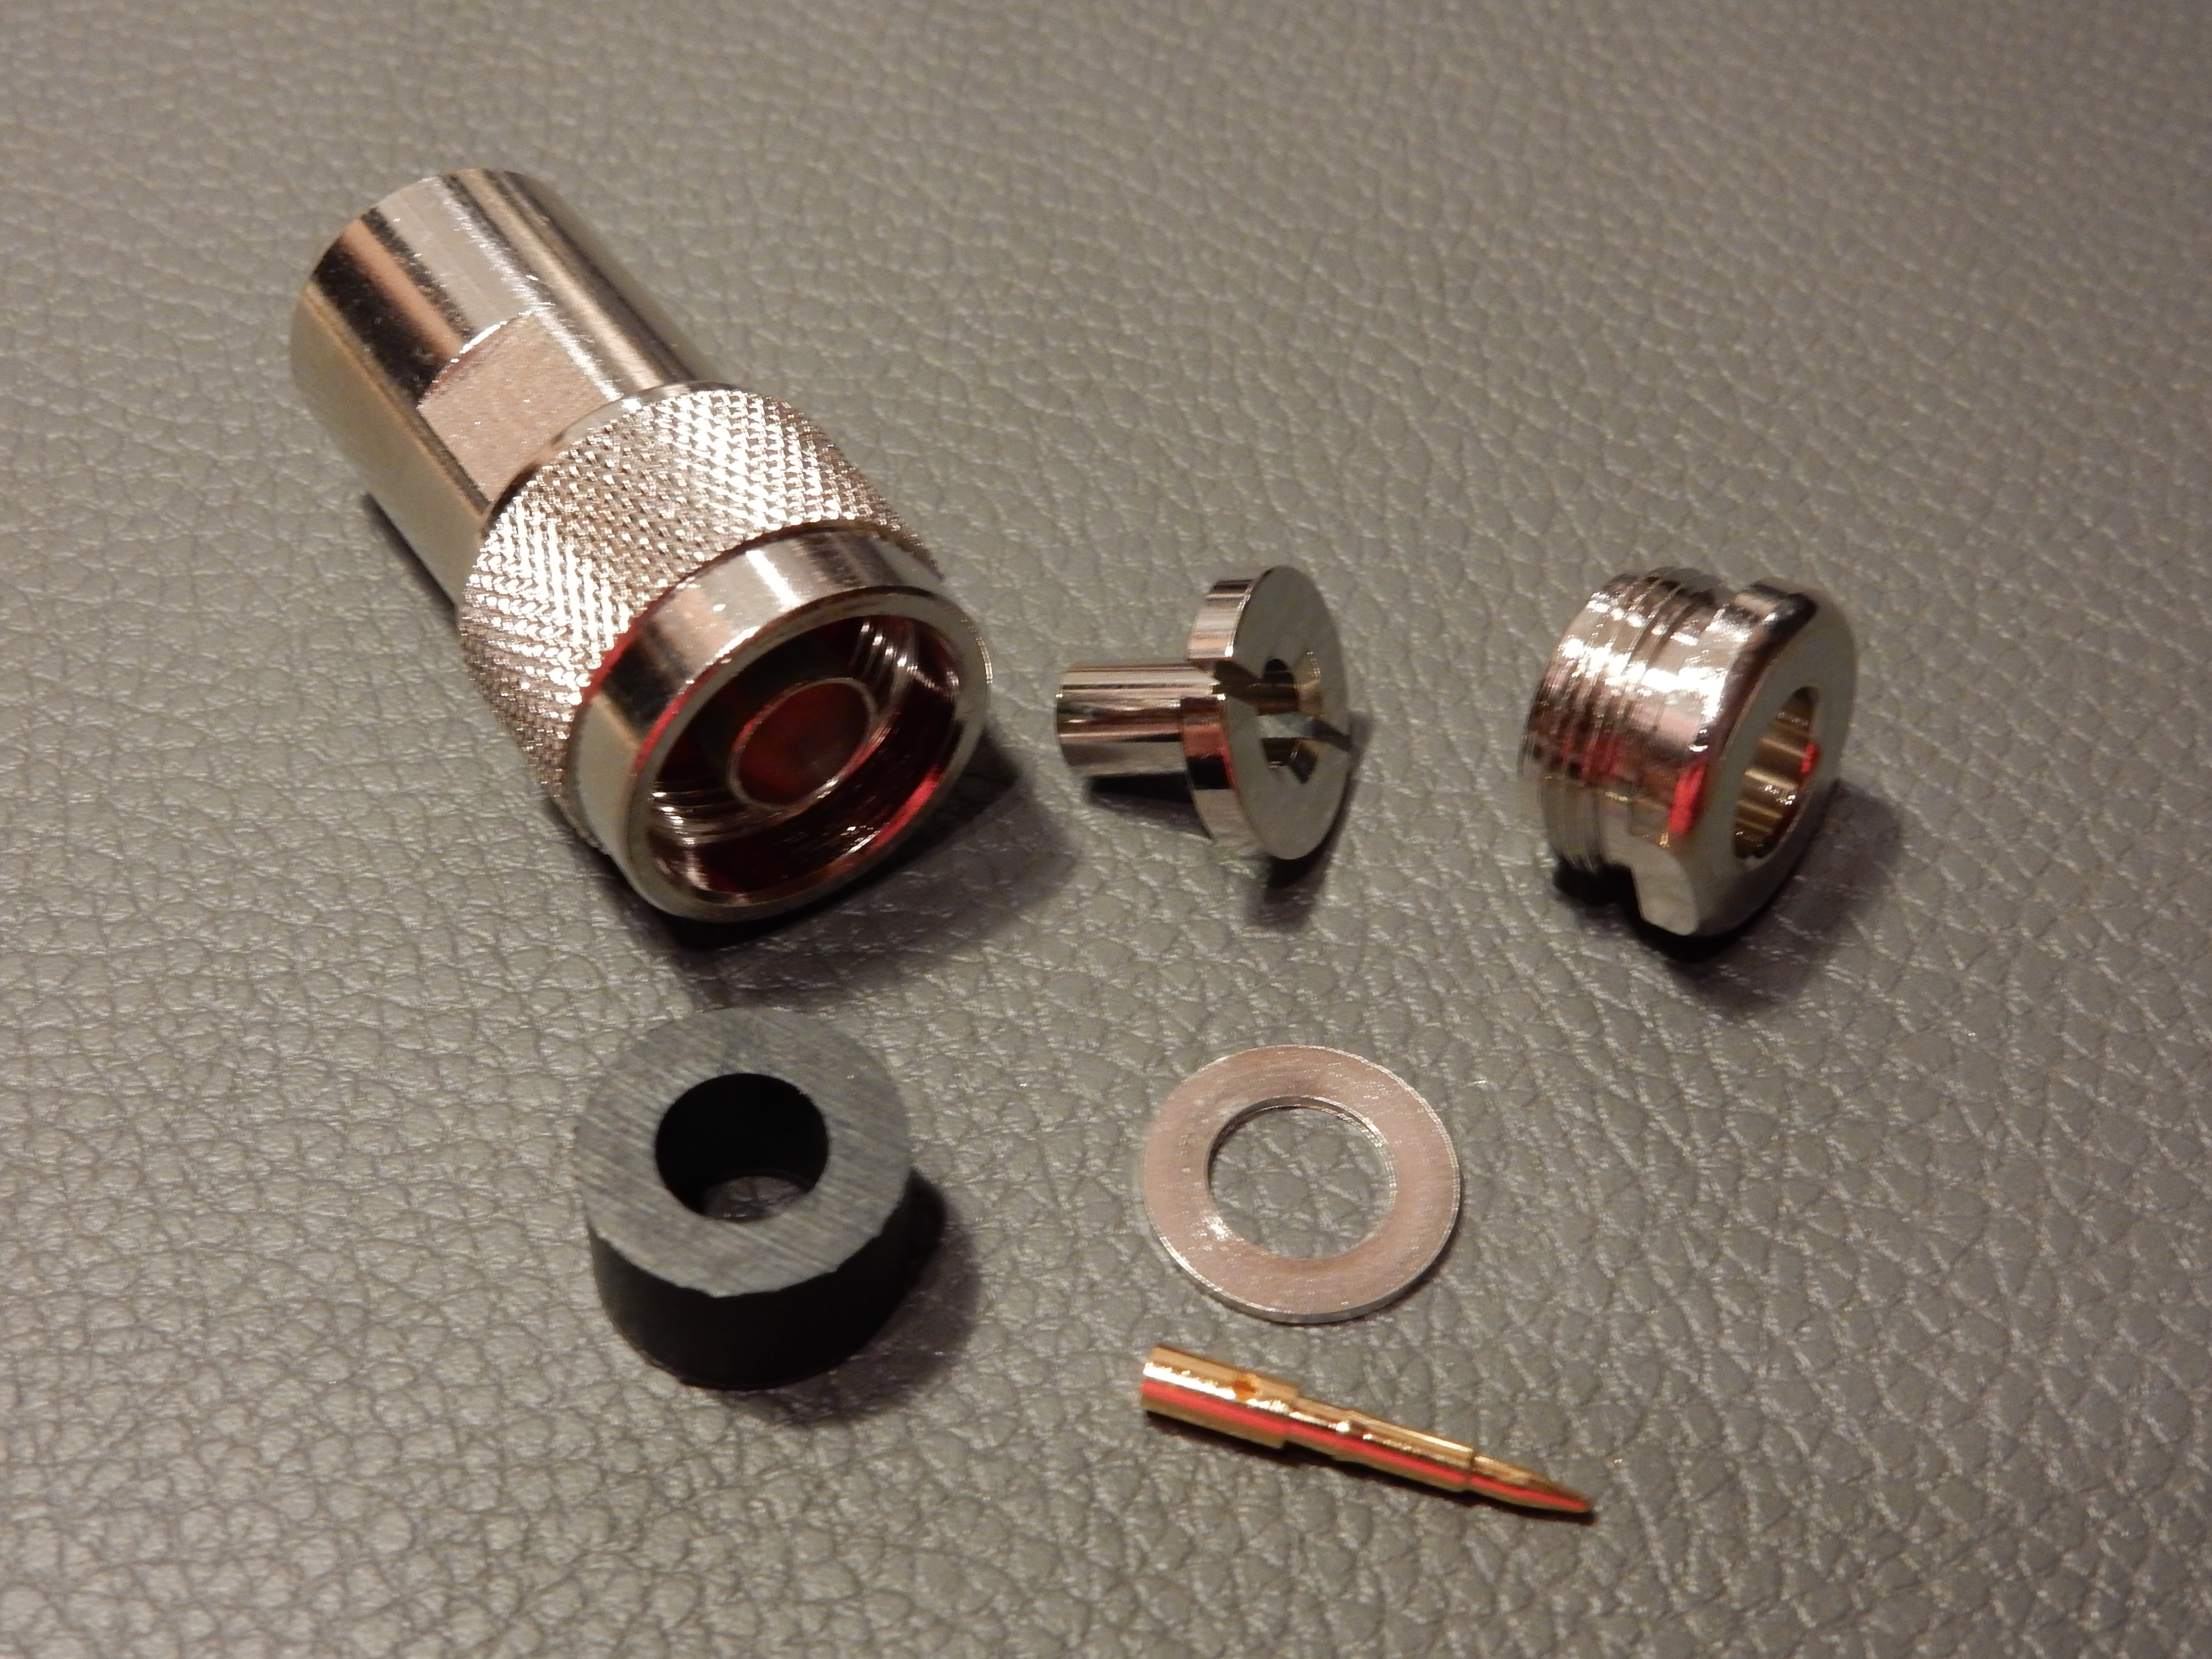
\includegraphics[width=0.85\textwidth]{foto/72}
    \caption{\scriptsize Ein N-Stecker vor seiner Montage}
    \label{n_koaxsteckverbinder_n_stecker}
\end{figure}

   \end{column}
\end{columns}

\end{frame}

\begin{frame}
\only<1>{
\begin{PQuestion}{NG204}{Welches HF-Steckverbindungs-System wird in der folgenden Darstellung gezeigt? }{SMA}
{PL}
{N}
{BNC}
{\DARCimage{1.0\linewidth}{610include}}\end{PQuestion}

}
\only<2>{
\begin{PQuestion}{NG204}{Welches HF-Steckverbindungs-System wird in der folgenden Darstellung gezeigt? }{SMA}
{PL}
{\textbf{\textcolor{DARCgreen}{N}}}
{BNC}
{\DARCimage{1.0\linewidth}{610include}}\end{PQuestion}

}
\end{frame}%ENDCONTENT
